\section{Objects of Analysis}
\label{sec:subjects}

We used \github{}'s search API~\cite{githubsearch} to identify
projects that satisfy the following criteria: (1) the primary language
is Java\footnote{In case of projects in multiple languages, the
  \github{} API considers the predominant language as the primary
  language.}, (2) the project has at least 100 stars, (3) the latest
update was on or after January 1st, 2016, and (4) the \emph{readme}
file contains the string \emph{mvn}.  We focused on Java for its
popularity.  Although there is no clearcut limit on the number of
\github{} stars~\cite{github-stars} to define relevant projects, we
observed that one hundred stars was enough to eliminate trivial subjects. The
third
criteria serves to skip projects without recent activity. The fourth
criteria is an approximation to find Maven projects.\Comment{ The
  rationale is that if the string \emph{mvn} exists in the
  \emph{readme} file, it may represent a Maven call (\eg, to compile
or to test the project).} We focused on Maven for its popularity on
Java projects.  Important to highlight that, as of now, the
\github{}'s search API can only reflect contents from repository
statistics (\eg, number of forks, main programming language); it does
not provide a feature to search for projects containing certain files
(\eg{}, \emph{pom.xml}) in the directory structure.
Figure~\ref{fig:subject-query} illustrates the query to the \github{}
API as an HTTP request.   The result set is sorted
in descending order of stars.

\begin{figure}[t!]
\centering
\tiny
\lstset{
    escapeinside={@}{@},
    numbers=left,xleftmargin=1em,frame=single,framexleftmargin=0.5em,
    basicstyle=\ttfamily\scriptsize, boxpos=c, numberstyle=\tiny,
    showstringspaces=false
}
\begin{lstlisting}
https://api.github.com/search/repositories?q=language:java
 +stars:>=100+pushed:>=2016+mvn%20in:readme&sort=stars
\end{lstlisting}
  \vspace{-3mm}
  \caption{\label{fig:subject-query} Query to the \github{} API for
  projects that (1) use Java, (2) contains at least 100
  stars, (3) has been updated on January 1st, 2016 (or later), (4) contains
  the string \emph{mvn} in the \emph{readme} file.}
  \vspace{-3mm}
\end{figure}

We used the following methodology to select projects for
analysis. After obtaining the list of potential projects from GitHub, we
filtered those
containing a \pomf{} file in the root directory.\Comment{  A Maven project may
contain several sub-modules with multiple \pomf{} files.}
Then, considering this set of Maven projects, we
executed the tests for \SubjectsReruns{} times to discard those projects with
issues
in the build file and non-deterministic results observed from sequential
executions.
As of August 25th 2017, our search criteria returned a total of
\SubjectsGithub{}
subjects.
From this set of projects,
\SubjectsGithubNotMaven{} projects were not Maven or did not have a
\pomf{} in the root directory, 
\SubjectsGithubNotTestable{} projects were not considered because of
environment incompatibility
(\eg, missing\Comment{ required web browser or database management
system}~DBMS),
\SubjectsGithubFlaky{} projects were discarded because of
``flaky tests''~\cite{luo-etal-fse2014}. A ``flaky'' test is a test that passes
or fails under
the same circumstances leading to non-deterministic results.
As some of our experiments consist of running tests on different
threads, we ignored these projects as it would be impractical
to identify whether a test failed due to a race condition or some
other source of flakiness.
From the remaining \SubjectsGithubConsistant{} projects with
deterministic results, we eliminated \SubjectsGithubTooManyFailures{}
projects with \SuiteFailingThreshold{} or more failing tests as to
reduce bias. For the
remaining projects with failing tests, we used the JUnit's
\CodeIn{@Ignore} annotation to ignore failing tests.
Our final set of subjects contains \numSubjs{} projects.
Figure~\ref{fig:subjects} summarizes our sample set.

\begin{figure}[ht]
  \vspace{-5mm}
  \centering
  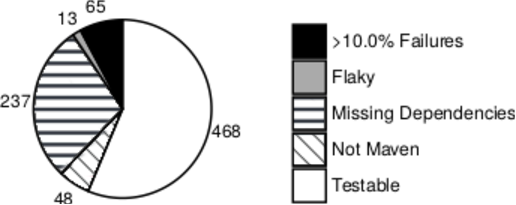
\includegraphics[width=0.27\textwidth]{results/piechart-subjs.pdf}
  \caption{\label{fig:subjects}We fetched \SubjectsGithub{} popular projects
  hosted on \github{}. From this initial sample, we ignored
  \SubjectsGithubNotMaven{} projects without Maven support,
  \SubjectsGithubNotTestable{} with missing dependencies,
  \SubjectsGithubFlaky{} projects with flaky tests, and
  \SubjectsGithubTooManyFailures{} projects had at least
  \SuiteFailingThreshold{} of failing tests. We considered
  \numSubjs{} projects to conduct our study.}
\end{figure}

\label{sec:setup}
To run our experiments, we used a Core i7-4790 (3.60 GHz) Intel processor
machine with eight virtual CPUs (four cores with two native threads each) and
16GB of memory, running Ubuntu 14.04 LTS Trusty Tahr (64-bit version).  We
used\Comment{ Git,} Java 8 and Maven 3.3.9 to build projects and run test
suites. To process test results and generate plots we used Python\Comment{ 3.4},
Bash, R and Ruby\Comment{ 2.3}.  All source artifacts are publicly available for
replication on our website~\cite{ourwebpage}.  This includes supporting
scripts\Comment{ (\eg, the scripts to run the tests and generate raw analysis
data)} and the full list of projects.

